\chapter{Functions}

\section{Sets}
Before defining what a function is or what it does, it is important to briefly discuss what goes into function and what comes out. Simply, \textit{sets}\index{set} are a collection of items and each one of those items are usually referred to as \textit{elements}\index{set!element}. Without getting into the weeds of set theory, sets can contain pretty much anything from numbers, functions, and other sets \cite{bookofproof}.

Some common sets that you may be familiar with are the \textit{natural numbers} $\N = \{1,2,3,4,5,\dots\}$, the \textit{integers} $\Z = \{\dots,-2,-1,0,1,2,\dots\}$, and the \textit{real numbers} $\R$, which is usually represented via a number line. Sets can also be intervals on the real line (i.e. [a,b) is an interval on $\R$ containing $a$ but not $b$) or even the possible results of flipping a coin $C = \{H,T\}$.

We will now define the basic notation when dealing with sets and the operations that can be performed on sets. We say that $x$ is an element of a set $A$ with the notation $x \in A$ and when $x$ is not in $A$, we say $x \not\in A$. For example, given the set $A = \{1,2,3,4\}$, we can say that $1 \in A$ is true as well as $5 \not\in A$.

The notion of combining sets comes with \textit{unions}\index{set!union} and \textit{intersections}\index{set!intersection}. Given $A$ and $B$ are sets, the union of $A$ and $B$ is denoted as $A \cup B$ and is equal to the set the contains elements in either $A$ or $B$. Similarly, the intersection between $A$ and $B$ is denoted as $A \cap B$ and is the set that contains elements that are in both $A$ and $B$. For example, given the sets $A = \{1,2,3,4\}$ and $B = \{3,4,5,6\}$, the union and intersection between $A$ and $B$ is

\begin{aequation}
    A \cup B &= \{1,2,3,4,5,6\} \\
    A \cap B &= \{3,4\}
\end{aequation}

Subsets are often used to relate different sets and their elements. A set $A$ is said to be a subset of another set $B$ if all of the elements of $A$ are also within $B$ and is denoted as $A \subseteq B$ and a set $A$ is equal to a set $B$ if and only if $A \subseteq B$ and $B \subseteq A$. An important subset is the empty set represented by the symbols $\varnothing$, $\emptyset$, or simply $\{\}$. It is important to note that the empty set is also a subset of all sets.

Using sets by listing them out can become cumbersome and sometimes confusing, instead set builder notation is used to build a set based on a rule. For example, the set of all positive even integers can be written as

\begin{equation}
    A = \{2,4,6,8,\dots\} = \{z : z \text{ is an positive even integer}\} = \{z : z = 2n, n\in\Z \text{ and } n > 0\}
\end{equation}

\noindent Here, the $:$ stands for "such that" which indicates the rule (the words "such that" or the symbol $|$ is also often used). The \textit{rational numbers} $\Q$ can also be constructed via the integers with

\begin{equation}
    \Q = \left\{\frac{p}{q} : p,q \in \Z \text{ and } q \neq 0\right\}
\end{equation}

As mentioned previously, intervals on the real number line can be represented as sets. Given two values $a$ and $b$ and assuming that $a \leq b$, intervals on the real line are represented as

\begin{itemize}
    \item Closed interval: $[a,b] = \{x \in \R : a \leq x \leq b\}$ \hfill \intervalinline{a}{b}{[}{]}
    \item Open interval: $(a,b) = \{x \in \R : a < x < b\}$ \hfill \intervalinline{a}{b}{(}{)}
    \item Half-open interval:
        \begin{itemize}
            \item $(a,b] = \{x \in \R : a < x \leq b\}$ \hfill \intervalinline{a}{b}{(}{]}
            \item $[a,b) = \{x \in \R : a \leq x < b\}$ \hfill \intervalinline{a}{b}{[}{)}
        \end{itemize}
    \item Infinite interval:
        \begin{itemize}
            \item $(a,\infty) = \{x \in \R: a < x\}$ \hfill \intervalinline{a}{$\infty$}{(}{}
                \item $[a,\infty) = \{x \in \R: a \leq x\}$ \hfill \intervalinline{a}{$\infty$}{[}{}
                \item $(-\infty,b) = \{x \in \R: x < b\}$ \hfill \intervalinline{$-\infty$}{b}{}{)}
            \item $(-\infty,b] = \{x \in \R: x \leq b\}$ \hfill \intervalinline{$-\infty$}{b}{}{]}
            \item $(-\infty,\infty) = \R$ \hfill \intervalinline{$-\infty$}{$\infty$}{}{}
        \end{itemize}
\end{itemize}

\noindent Here, the open brackets $($ and $)$ indicate that the respective endpoint is not included, while the closed brackets $[$ and $]$ indicate that the respective endpoint is included in the interval.

The \textit{Cartesian product}\index{set!Cartesian product} (also known as the \textit{direct product}\index{set!direct product}) is used often to describe ordered pairs or even higher-dimension coordinates. Some examples include the $xy$-plane also known as $\R^2$, 3D space with $\R^3$. The Cartesian product for two sets $A$ and $B$ is defined as

\begin{equation}
    A \times B = \{(a,b) : a \in A, b \in B\}
\end{equation}

\noindent Note that, in general, $A \times B \neq B \times A$ as the operation is order dependent. Higher-order products are defined with sets $A_1, A_2, \dots, A_n$ as

\begin{equation}
    A_1 \times A_2 \times \cdots \times A_n = \{(a_1,a_2,\dots,a_n): a_i \in A_i, i \in \{1,2,\dots,n\}\}
\end{equation}

\noindent As previously mentioned, the 2D plane as well as the 3D plane can be constructed using Cartesian products as well and is done as such with the set of real numbers $\R$

\begin{aequation}
    \R^2 &= \R \times \R = \{(x,y): x,y \in \R\}\\
    \R^3 &= \R \times \R \times \R = \{(x,y,z): x,y,z \in \R\}\\
    & \vdots \\
    \R^n &= \R \times \R \times \dots \times \R = \{(x_1, x_2, \dots, x_n) : x_i \in \R, i \in \{1,2,\dots, n\} \}
\end{aequation}

For further and more formal discussion on sets and naive set theory as well as formal logic and proof writing, refer to \cite{naivesettheory} or \cite{bookofproof}.

\subsection{Exercises}

\section{What is a function?}
\textit{Functions}\index{function} are objects in math that describe a relationship or mapping between two sets. Given two sets $X$ and $Y$, a function $f$ maps the unique elements of $X$, called the \textit{domain}\index{function!domain} of the function, to elements in the set $Y$ called the \textit{codomain}\index{function!codomain} of the function and the relationship is denoted as $f : X \to Y$ ("$f$ maps from $X$ to $Y$") or $y = f(x)$ ("$y$ equals $f$ of $x$" \cite{understandinganalysis}), where $y \in R \subseteq Y$ is known as the \textit{dependent variable}\index{function!dependent variable} with $R$ as the range of the function and $x \in X$ is known as the \textit{independent variable}\index{function!independent variable} or the \textit{argument}\index{function!argument} of the function. The \textit{range}\index{function!range} of a function is the set of all possible values that $f(x)$ is able to output with $X$ as its domain, note that the range is a subset of the codomain $Y$ but is not always equal. Formally, the definition is as follows

\begin{definition}
    A \textit{function} is a mapping or rule that assigns each element from a set called the domain $X$ of the function to a unique element in the range $R = f(X)$ of the function which is a subset of the codomain $R \subseteq Y$ and the element $x \in X$ is mapped to an element in $y \in R \subseteq Y$ with $x \mapsto y$.
\end{definition}

Further emphasis must be made on the elements $y = f(x)$. The function $f(x)$ maps the element $x \in X$ to exactly one element $y \in Y$ \cite{elemrealandcomplex}. For single variable functions, this can be tested using the vertical line test on a function's graph (covered shortly). If a formula results in two answers with one input (i.e. the equation for a circle: $x^2 + y^2 = r$ gives two points of $y$ for each $x$) it is no longer considered a function. Figure \ref{functionmapping} shows how a function maps elements of the domain to the range.

\begin{figure}[!ht]
    \centering
    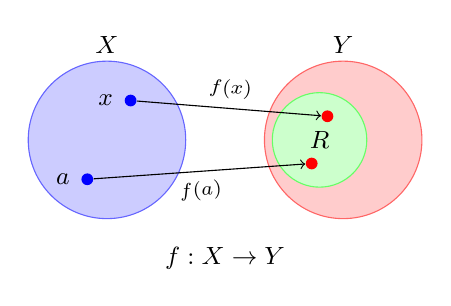
\begin{tikzpicture}[font=\small]
        % % Origin (for reference)
        % \node (origin) at (0,0) {$\bullet$};

        % Domain (X) - Blue circle
        \filldraw[fill=blue!20, draw=blue!60] (-1.5,0) circle (1cm);
        \node at (-1.5,1.2) {$X$};  % Domain label above circle

        % Codomain (Y) - Red circle with Range (R) - Green circle
        \filldraw[fill=red!20, draw=red!60] (1.5,0) circle (1cm);
        \node at (1.5,1.2) {$Y$};  % Codomain label above circle
        \filldraw[fill=green!20, draw=green!60] (1.2,0) circle (0.6cm);
        \node at (1.2,0) {$R$};  % Range label centered in green circle

        % Domain points with tight labels
        \node[circle,fill=blue,inner sep=1.5pt] (x) at (-1.2,0.5) {};
        \node[left=0.1cm] at (x) {$x$};

        \node[circle,fill=blue,inner sep=1.5pt] (a) at (-1.75,-0.5) {};
        \node[left=0.1cm] at (a) {$a$};

        % Codomain points
        \node[circle,fill=red,inner sep=1.5pt] (fx) at (1.3,0.3) {};
        \node[circle,fill=red,inner sep=1.5pt] (fa) at (1.1,-0.3) {};

        % Arrows with labels attached
        \draw[->] (x) -- node[midway,above,sloped] {\scriptsize$f(x)$} (fx);
        \draw[->] (a) -- node[midway,below,sloped] {\scriptsize$f(a)$} (fa);

        % Function label below
        \node at (0,-1.5) {$f: X \to Y$};
    \end{tikzpicture}
    \caption{Function mapping diagram showing the domain $X$, codomain $Y$, and range $f(X)$}
    \label{functionmapping}
\end{figure}

\begin{example}
    Some real-world examples of functions are
    \begin{itemize}
        \item The area of a circle: \dotfill $A(r) = \pi r^2$
        \item The height of a falling ball: \dotfill $h(t) = h_0 + v_0 t - (1/2)gt^2$
        \item Compound interest: \dotfill $A(t) = P(1+\frac{r}{n})^{nt}$
        \item Temperature conversion: \dotfill $C(F) = \frac{5}{9}(F - 32)$
        \item %TODO: add more examples here
    \end{itemize}
    It can be useful to think of functions as machines that take in an input and produces an output. The examples above show such cases using mathematical formulas that give a set of instructions on how the input is transformed from the element in the domain to the element in the range.
\end{example}

\subsection{Graphs of Functions}

Another way to represent functions is with its \textit{graph}\index{function!graph} which is a set of points consisting of the input and its corresponding output and is represented with the set of ordered pairs $\{(x,y) : y = f(x), x\in\R\}$ for functions that accept real numbers.

\begin{example}
    A familiar example is the linear function $f(x) = mx + b$ where $m$ is the slope of the line and $b$ is the vertical offset. Suppose $m = 1$ and $b = 0$, we get the following graph for the function $f(x) = x$ in Figure \ref{f(x)=x graph}
    \begin{figure}[!ht]
        \centering
        \begin{tikzpicture}
            \begin{axis}[xmin=-2, xmax=2, ymin=-2, ymax=2,
                axis lines=middle, xlabel=$x$, ylabel=$y$]
                \addplot[color=black,grid,]{x};
            \end{axis}
        \end{tikzpicture}
        \label{f(x)=x graph}
        \caption{Graph of the function $f(x) = x$}
    \end{figure}
\end{example}

\begin{example}
    Another example is the quadratic function of the form $f(x) = ax^2 + bx + c$, where $a,b,c \in \R$ are the coefficients of the function and determine its shape. Suppose that $a = 1, b = 0, c = -1$ resulting in the function $f(x) = x^2 - 1$. Using knowledge of the roots a quadratic function, it can be deduced that this will result in a parabola with $x$-intersections at $x = -1$ and $x = 1$ which can be confirmed in the graph in Figure \ref{f(x)=x^2-1graph}

    \begin{figure}[!ht]
        \centering
        \begin{tikzpicture}
            \begin{axis}[
                    xmin=-2, xmax=2,
                    ymin=-2, ymax=2,
                    xlabel=$x$, ylabel=$y$,
                    axis lines=middle,
                    % grid=both
                ]
                \addplot[color=black, domain=-2:2, samples=50]{x^2 - 1};
            \end{axis}
        \end{tikzpicture}
        \label{f(x)=x^2-1graph}
        \caption{Graph of the function $f(x) = x^2-1$}
    \end{figure}
\end{example}

\subsection{Table Functions}

The last representation of a function that will be discussed are functions that are in the form of tables. Consider two finite sets $X = \{1,2,3,4,5\}$ and $Y = \{2,4,6,8,10\}$ and a function that maps the elements of $X$ to the elements of $Y$. A table can be created that shows the assignment of the elements (Table \ref{tab:tablefunctionex}) via the function $f(x)$.

\begin{table}[!ht]
    \centering
    \[
        \begin{array}{|*{6}{c|}}
            \hline
            x \in X & 1 & 2 & 3 & 4 & 5 \\
            \hline
            y \in Y & 2 & 4 & 6 & 8 & 10 \\
            \hline
        \end{array}
    \]
    \caption{Function Mapping from \( X \) to \( Y \)}
    \label{tab:tablefunctionex}
\end{table}

The function shown in Table \ref{tab:tablefunctionex} is constructed from a mathematical formula ($y = 2x$), this is not necessary, as long as there is only one output for any given input, then, the table is considered a function.

\begin{example} For example, consider the following table that shows the function that maps $X = \{1,3,5,8,4\}$ to $Y = \{3,5,2,1,1\}$ in Table \ref{tab:tablefunctionex2}.
    \begin{table}[!ht]
        \centering
        \[
            \begin{array}{|*{6}{c|}}
                \hline
                x \in X & 1 & 3 & 5 & 8 & 4 \\
                \hline
                y \in Y & 3 & 5 & 2 & 1 & 1 \\
                \hline
            \end{array}
        \]
        \caption{Function Mapping from \( X \) to \( Y \)}
        \label{tab:tablefunctionex2}
    \end{table}
    Though a value in $Y$ repeats once, it still passes the vertical line test as the function maps only one output $y$ from any input $x$.
\end{example}

This conceptual foundation of what a  function is prepares us for the introduction and review of commonly used functions and function families (functions with similar forms and properties).

\subsection{Exercises}

\section{Common Functions}
Functions, namely those defined via mathematical formulas, can be classified into function families whose members share common features, forms, and properties. Some such families often differ only in coefficients and others may change the base in which they operate. The following types of functions are used frequently in the study of calculus.

\subsection{Linear Functions}
Beginning with the most elementary form of functions created using mathematical formulas is the \textit{linear function}\index{function!linear} or the equation for a line.

\begin{definition}
    Functions of the form $f(x) = mx + b$, where $m$ is the slope and $b$ is the $y$-intercept, are \textit{linear functions}.
\end{definition}

The graphs of linear functions are straight lines, if the domain of the function is $\R$, then the graph of $f$ extends from $-\infty$ to $+\infty$. It's slope determines the angle of the line and can be reconstructed with any two points on the line with the following formula

\begin{equation}
    m = \frac{y_2-y_1}{x_2-x_1}
    \label{slopeofaline}
\end{equation}

\noindent where $y_i$ corresponds to $x_i$ and $x_2 > x_1$. The $y$-intercept the value of the $y$-coordinate of the function when $x=0$ and denotes where the line crosses the $y$-axis on the graph. An example for the graph of a linear function is shown in Figure \ref{f(x)=x graph} where $f(x) = x$.

\begin{example}
    Linear functions can model the conversion between temperatures in degrees Celsius and Fahrenheit with the function $C(F) = \frac{5}{9}(F - 32) = \frac{5}{9}F - \frac{160}{9}$. Here the independent variable is F, the slope is $\frac{5}{9}$, and the $y$-intercept is $\frac{160}{9}$ and the graph is shown in Figure \ref{FtoCgraph}.

    \begin{figure}[!ht]
        \centering
        \begin{tikzpicture}
            \begin{axis}[xmin=-10, xmax=40, ymin=-20, ymax=10,
                axis lines=middle, xlabel=$F$, ylabel=$C(F)$]
                \addplot[color=black,grid,domain=-10:40]{5/9*(x-32)};
            \end{axis}
        \end{tikzpicture}
        \label{FtoCgraph}
        \caption{Graph of the Fahrenheit to Celsius Conversion, $C(F) = \frac{5}{9}(F-32)$}
    \end{figure}
\end{example}

% TODO: add more discussion here

\subsection{Quadratic Functions}
Quadratic functions are the next natural progression after linear functions. The simplest form of a quadratic function $f(x) = x^2$ consists of $x$ multiplied by itself. The graph of a quadratic equation is a \textit{parabola}\index{function!quadratic!parabola} and can be seen in Figure \ref{f(x)=x^2-1graph}.

\begin{definition}
    Functions of the form $f(x) = ax^2 + bx + c$ are \textit{quadratic functions}\index{function!quadratic}, this is the standard form for a quadratic function. Alternative forms to the standard quadratic function are the root form $f(x) = (x-a)(x-b)$ where $a$ and $b$ are the $x$-intercepts of the function and the vertex form $f(x) = a(x-h)^2+k$ where the point $h,k$ is the vertex of the parabola.
\end{definition}

Quadratic functions have some useful properties such as the root(s) of the parabola (the $x$-intercept(s)) as well as having an explicit formula for computing the root(s) of the function known as the \textit{quadratic formula}\index{function!quadratic!formula}. The quadratic formula solves for the $x$-coordinate(s) of the roots for a given quadratic function (where $y=0$)

\begin{equation}
    x = \frac{-b \pm \sqrt{b^2 - 4ac}}{2a}
\end{equation}

\noindent where $a$, $b$, and $c$ are the coefficients in the standard form of a quadratic function. This forumla gives real roots when the \textit{discriminant}\index{function!quadratic!discriminant} $b^2 - 4ac > 0$, a single real root (with a multiplicity of two) when $b^2 - 4ac = 0$, complex roots when $b^2 - 4ac < 0$, and purely imaginary roots when $b = 0$ and $4ac > 0$.

\begin{example}
    An example of a quadratic function is \textit{vertical projectile motion} under gravity:

    \noindent Given an object with initial height $h_0$ and initial vertical velocity $v_0$, its height at time $t$ is modeled by

    \begin{equation}
        h(t) = -\frac{1}{2}gt^2 + v_0 t + h_0
    \end{equation}

    \noindent where $h(t)$ is the height at time $t$, $g$ is the the acceleration due to gravity ($g \approx 9.81 \text{m/s}^2$) at Earth's surface, and air resistance is neglected. The graph showing the height of a particle thrown from a height of $20$ meters and at an initial vertical velocity of $2$ m/s$^2$ is shown in Figure \ref{ballistictrajectory}.

    \begin{figure}[!ht]
        \centering
        \begin{tikzpicture}
            \begin{axis}[xmin=-1, xmax=3, ymin=-1, ymax=25,
                axis lines=middle, xlabel=$t$, ylabel=$h(t)$]
                \addplot[color=black,grid,domain=0:10,samples=75]{-1/2*9.81*x^2 + 2*x + 20};
            \end{axis}
        \end{tikzpicture}
        \label{ballistictrajectory}
        \caption{Graph of a Particle Falling Due to Gravity over time, $h(t) = -\frac{1}{2}gt^2 + v_0 t + h_0$}
    \end{figure}
\end{example}

\subsection{Polynomial and Rational Functions}
Generalizing upon the linear and quadratic functions further, polynomial functions are the next step.

\begin{definition}
    Functions of the form $f(x) = a_n x^n + a_{n-1} x^{n-1} + \cdots + a_2 x^2 + a_1 x + a_0$ are \textit{polynomial functions}\index{function!polynomial}. Where $n$ is the \textit{degree}\index{function!polynomial!degree} of the polynomial (whne $a_n \neq 0$) and $a_i$ for $i \in {0,1,\dots,n-1,n}$ are the coefficients.
\end{definition}

Similar to quadratic functions, polynomials have up to $n$ roots but do not have an explicit formula to compute those roots for polynomials with degree $n > 3$. Linear functions and quadratic functions can be considered special cases of polynomial functions with degree $n=1$ and $n=2$ respectively. Common higher-order polynomials are \textit{cubic functions}\index{function!polynomial!cubic} $n=3$, \textit{quartic functions}\index{function!polynomial!quartic} $n=4$, and \textit{quintic functions}\index{function!polynomial!quintic} $n=5$. A useful property of polynomials is that there are at most $n$ roots for a polynomial of degree $n$, note that when a polynomial has less (real and complex) roots than its degree, one of its roots may have a multiplicity greater than one meaning that it is repeated. For example, the polynomial (in root form) $f(x) = (x+1)(x+1)(x+1) = (x+1)^3 = x^3 + 3x^2 + 3x + 1$ has all three roots at $x=-1$ which means that the root $(x=-1,y=0)$ has multiplicity of 3.

\begin{example} To show the differences between polynomials with varying order, Figure \ref{fig:polynomials} graphs polynomials of the form $x^n$ up to the $6$th degree.

    \begin{figure}[!ht]
        \centering
        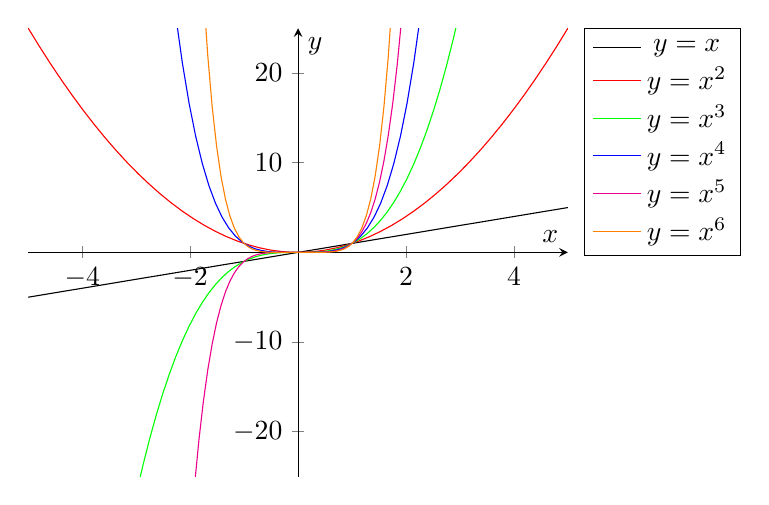
\begin{tikzpicture}
            \begin{axis}[
                    xmin=-5, xmax=5,
                    ymin=-25, ymax=25,
                    axis lines=middle,
                    xlabel=$x$,
                    ylabel=$y$,
                    % grid=both,
                    legend pos=outer north east,
                    % title={Polynomial Functions}
                ]
                \addplot[color=black, domain=-5:5, samples=2]{x};
                \addplot[color=red, domain=-5:5, samples=50]{x^2};
                \addplot[color=green, domain=-3:3, samples=50]{x^3};
                \addplot[color=blue, domain=-3:3, samples=50]{x^4};
                \addplot[color=magenta, domain=-2:2, samples=50]{x^5};
                \addplot[color=orange, domain=-2:2, samples=50]{x^6};
                \legend{$y = x$, $y = x^2$, $y = x^3$, $y = x^4$, $y = x^5$, $y = x^6$}
            \end{axis}
        \end{tikzpicture}
        \caption{Polynomials of varying degrees $n \in \{1,2,3,4,5,6\}$}
        \label{fig:polynomials}
    \end{figure}
\end{example}

Rational functions branch from polynomials in a similar way to how rational numbers branch from the integers as they are constructed by dividing one polynomial by another.

\begin{definition}
    The function of the form $f(x) = \frac{p(x)}{q(x)}$ where $p(x)$ and $q(x) \neq 0$ are polynomial functions are known as \textit{rational functions}\index{function!rational}.
\end{definition}

Like polynomials, rational functions have \textit{zeros}\index{function!rational!zeros} or roots when the numerator is equal to zero, but also zeros when the denominator of the function is equal to zero called \textit{poles}\index{function!rational!poles}. These describe discontinuous points as the the denominators reach zero resulting in holes (when a zero and a pole cancel) and an \textit{asymptote}\index{function!rational!asymptote} when the pole is not cancelled.

\begin{example} An example of a rational function that has both holes and asymptotes is
    \begin{equation}
        f(x) = \frac{(x-1)(x+1)(x+2)}{(x-1)(x+1)(x-2)}
    \end{equation}

    \noindent This function has holes at $x = \pm 1$ where the poles and zeros cancel out asymptotes at $x = 2$ where the denominator becomes zero and $y = 1$ for the horizontal asymptote. The graph for this function is shown in Figure \ref{fig:rationalholeandasymptote}.

\begin{figure}[!ht]
    \centering
    \begin{tikzpicture}
        \begin{axis}[
                xmin=-7, xmax=7,
                ymin=-7, ymax=7,
                axis lines=middle,
                xlabel=$x$,
                ylabel=$y$,
                legend pos=outer north east,
                restrict y to domain=-10:10, % Prevents asymptote overflow
            ]
            \draw[dashed, red] (axis cs:2,-7) -- (axis cs:2,7);
            \draw[dashed, blue] (axis cs:-7,1) -- (axis cs:7,1);
            
            \addplot[color=black, domain=-7:1.99, samples=50, unbounded coords=jump]
                {(x-1)*(x+1)*(x+2)/((x-1)*(x+1)*(x-2)};
            \addplot[color=black, domain=2.01:7, samples=50, unbounded coords=jump]
                {(x-1)*(x+1)*(x+2)/((x-1)*(x+1)*(x-2)};
            
            % Holes at x=1 and x=-1
            \addplot[only marks, mark=*, mark options={fill=white, draw=black}]
                coordinates {
                    (1, -3)    % Hole at x=1 (lim_{x→1} f(x) = -3)
                    (-1, -1/3) % Hole at x=-1 (lim_{x→-1} f(x) = -1/3)
                };
        \end{axis}
    \end{tikzpicture}
    \caption{Rational function $f(x) = \frac{(x-1)(x+1)(x+2)}{(x-1)(x+1)(x-2)}$ with holes at $(1,-3)$ and $(-1,-\frac{1}{3})$, vertical asymptote at $x=2$, and horizontal asymptote at $y=1$}
    \label{fig:rationalholeandasymptote}
\end{figure}
\end{example}

\subsection{Trigonometric Functions}
Breaking away from the progression found from starting with linear functions and ending with polynomials

\subsection{Power, Exponential, and Logarithmic Functions}
\subsection{Systems of Equations}

\section{Types of Functions}
It is important to be able to distinguish functions and classify their behaviors into distinct characteristics in order to properly analyze them. Characteristics such as symmetry (evenness and oddness of a function) and periodicity (repeating functions) are defined in such ways that may give insight into solving certain problems or giving us the opportunity to exploit their definitions.

\subsection{Piecewise Functions and Absolute Values}
\subsection{Even and Odd Functions}
\begin{definition}
    A function $f(x)$ is said to be an \textit{even function}\index{function!even} of the independent variable $x$ if and only if
    $$
    f(-x) = f(x)
    $$
    for all $x$ in the function's domain.
\end{definition}

\begin{definition}
    A function $f(x)$ is said to be an \textit{odd function}\index{function!odd} of the independent variable $x$ if and only if
    $$
    f(-x) = -f(x)
    $$
    for all $x$ in the function's domain.
\end{definition}

\subsection{Increasing and Decreasing Functions}
\begin{definition}
    A function $f$ is \textit{increasing}\index{function!increasing} on an interval $I$ if for all $x_1, x_2 \in I$ with $x_1 < x_2$,
    $$
    f(x_1) \leq f(x_2).
    $$
    If the inequality is strict ($f(x_1) < f(x_2)$), we say $f$ is \textit{strictly increasing}\index{function!strictly increasing}.
\end{definition}

\begin{definition}
    A function $f$ is \textit{decreasing}\index{function!decreasing} on an interval $I$ if for all $x_1, x_2 \in I$ with $x_1 < x_2$,
    $$
    f(x_1) \geq f(x_2).
    $$
    If the inequality is strict ($f(x_1) > f(x_2)$), we say $f$ is \textit{strictly decreasing}\index{function!strictly decreasing}.
\end{definition}

\subsection{Periodic Functions}
\begin{definition}
    A function is said to be a \textit{period function}\index{function!periodic} if and only if for some value $a$,
    $$
    f(x) = f(x+a)
    $$
    where $a$ is the period of the function. The period defines the magnitude of the independent variable required for the function to repeat.
\end{definition}

\section{Function Transformations and Operations}
\subsection{Function Arithmetic}
\subsection{Function Translation}
\subsection{Fuction Composition}
\subsection{Function Inverses}
